%
%
\chapter{Compuation of the retarded Green Function}
\label{appch:green function}
%
%
The computation of the Green function $\mathcal{G}_{\dot{\mt{P}}\dot{\mt{P}}}(\vb{k}, z)$ in \eqref{eq:static conductivity formula} is displayed in detail in the following appendix.
The Green function is given by equation \eqref{eq:Green function}.
For using the diagrammatic technique the integral is transformed into Matsubara time $\tau = it$.
The magnitude of the Jacobi determinate is $-i$ and the upper limit is changed to $\beta = T^{-1}$.
Each time derivative is further generated an imaginary unit $i$.
The Green function is represented in Matsubara time as
%
\begin{align}
	\mathcal{G}_{\dot{\mt{P}}\dot{\mt{P}}}(\vb{k}, z) = i \int\limits_{0}^{\beta} \dd{\tau} e^{z \tau} \expval{\mathcal{T}_{\tau} \dot{\mt{P}}_{j}(\tau) \dot{\mt{P}}_{j}(0)}_{\mt{H}}.
\end{align}
%
$z$ is a complex frequency and the direction of the momentum is marked by the index $j = x,y$.
The index $H$ denotes, that the expectation value is evaluated with respect to Hamiltonian $\mt{H} = \mt{H}_{\Psi} + \mt{H}_{\Phi} + mt{H}_{\Psi\Phi}$, where the interaction between fermions and spin fluctuations is considered by the last term.
In Matsubara interaction representation, the appearing time evoluation operator is expanded up the the zeroth order.
As a consequance, corrections of the Green function, caused by the fermion-spin fluctuation interaction, are neglected.
Only the two time derivatives of momentum are therefore contained in the expectation value.
This is the only origin, where the pertubation of umklapp scattering is considered.
The Green function is given by
%
\begin{align}
	\mathcal{G}_{\dot{\mt{P}}\dot{\mt{P}}}(\vb{k}, z) = i \int\limits_{0}^{\beta} \dd{\tau} e^{z \tau} \expval{\mathcal{T}_{\tau} \dot{\mt{P}}_{j}(\tau) \dot{\mt{P}}_{j}(0)}_{\mt{H}_{0}}
\end{align}
%
where the expectation value is now evaluated with respect to the free Hamiltonian $\mt{H}_{0} = \mt{H}_{\Psi} + \mt{H}_{\Phi}$.
The time derivative of momentum is designated in equation \eqref{eq:time derivative momentum finite}.
Inserting this expression, $\mathcal{G}_{\dot{\mt{P}}\dot{\mt{P}}}(\vb{k}, z)$ is given by
%
\begin{align}
	\mathcal{G}_{\dot{\mt{P}}\dot{\mt{P}}}(\vb{k}, z) &= 
		-i 
		\sum\limits_{\mu, \lambda}
		\sum\limits_{\vb{G}_{1}, \vb{G}_{2}} 
		\mt{J}_{\vb{G}_{1}} \mt{J}_{\vb{G}_{2}} 
		\int\limits_{0}^{\beta} \dd{\tau} e^{z \tau} 
		\int_{\vb{k}_{1}}\int_{\vb{k}_{2}} G_{1,j}  G_{2,j} 
		\notag \\
		&\times
		\expval{\mathcal{T}_{\tau} \Phi_{\mu}(\vb{k}_{1},\tau) \Phi_{\mu}(-\vb{k}_{1} - \vb{G}_{1},\tau) \Phi_{\lambda}(\vb{k}_{2},0) \Phi_{\lambda}(-\vb{k}_{2} - \vb{G}_{2},0)}_{\mt{H}_{0}}.
\end{align}
%
Here, the moment integrals are extended over the first Brillouin zone, while the sum over $\vb{G}_{1}$ and $\vb{G}_{2}$ runs over all reciprocal lattice vectors.
$\vb{G}_{i}$, where $i=1,2$, is the coupling parameter with respect to the reciprocal lattice vector.
The sum over $\mu$ and $\lambda$ runs over the spatial direction of the three component bosonic field, while the direction of P is indicated by $j$.

Wick's theorem is used to seperate the expectation value in terms of free propagators.
Three contraction are possible for a an expectation value, including four bosonic, real field operators.
One of them is not contributed, since the operators to equal times are contracted.
The remaining two diagrams are both bubble diagrams and topological equivalent.
The diagram is depicted in figure \ref{fig:spin wave bubble}.

Acting Wick's theorem in momentum representation, each interchange of the bosonic operators yields a $\delta$-distribution, or more presicely, the  commutator relation.
This signifies the momentum conservation at each vertex.
One momentum integral one sum over reciprocal lattice vector and the sum over $\lambda$ are therefore evaluated directly.
The remaining vectors are renamed into $\vb{k}$ and $\vb{G}$ for the momentum and reciprocal lattice vector, respectivily.
%
%\begin{figure}
%	\centering
%	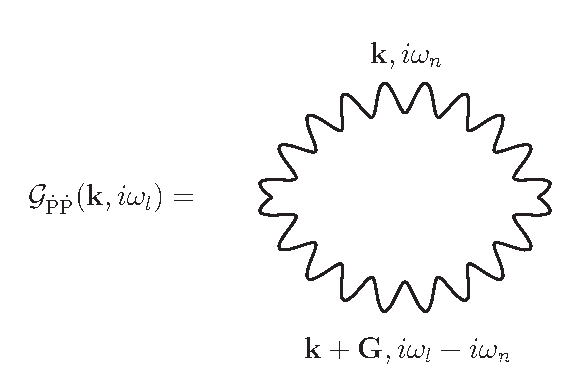
\includegraphics[width=0.5\textwidth]{spin_wave_bubble.eps}
%	\caption{}
%	\label{fig:spin wave bubble}
%\end{figure}
%
%
\begin{align}
	\mathcal{G}_{\dot{\mt{P}}\dot{\mt{P}}}(\vb{k}, z) &= 
		-2 
		\sum\limits_{\vb{G}} 
		\vert \mt{J}_{\vb{G}} \vert^{2}
		\int\limits_{0}^{\beta} \dd{\tau} e^{z \tau} 
		\int_{\vb{k}} G_{j}^{2}
		\notag \\
		&\times
		\expval{\mathcal{T}_{\tau} \Phi_{\mu}(\vb{k},\tau) \Phi_{\mu}(-\vb{k},0)}_{\mt{H}_{0}} 
		\expval{\mathcal{T}_{\tau} \Phi_{\mu}(-\vb{k} - \vb{G},\tau) \Phi_{\mu}(\vb{k}+\vb{G},0)}_{\mt{H}_{0}},
\end{align}
%
The factor of 2 is originated by the sum over both identical diagrams.
Furthermore, the relation $\mt{J}_{-\vb{G}} = \mt{J}_{\vb{G}}^{*}$ is used, where the complex conjugated is denoted by the asterisk.
The obtained expectation values are the free spin density propagtors $\mathcal{D}_{\mu}^{(0)}(\vb{k},\tau)$.
Both propagators are transformed into Matsubara frequency space, using the transformation rule
%
\begin{align}
	\mathcal{D}_{\mu}^{(0)}(\vb{k},\tau) = \frac{1}{\beta} \sum\limits_{\omega_{n}} e^{-i\omega_{n}\tau} \mathcal{D}_{\mu}^{(0)}(\vb{k},i\omega_{n})
\end{align}
%
where the summation runs over all bosonic Matsubara frequencies $\omega_{n} = \flatfrac{2n\pi}{\beta}$, where $n\in\mathbb{Z}$.
The frequency argument of the Green function is set to $z = i\omega_{l}$, since the Green function is now investigated onto the imaginary frequency axis.
The exponential functions are generated the only $\tau$-dependence and the $\tau$-integral is evaluated to $\beta \delta_{\omega_{m}+\omega_{l}-\omega_{n}}$.
One of the two sums over Matsubara frequencies is evaluated as well.
The following expression is obtained:
%
\begin{align}
	\mathcal{G}_{\dot{\mt{P}}\dot{\mt{P}}}(\vb{k}, i\omega_{l}) &= 
		-2 
		\sum\limits_{\vb{G}} 
		\vert \mt{J}_{\vb{G}} \vert^{2}
		\int_{\vb{k}} G_{j}^{2}
		\frac{1}{\beta} \sum\limits_{\omega_{n}}
		\mathcal{D}_{\mu}(\vb{k},i\omega_{n}) \,
		\mathcal{D}_{\mu}(-\vb{k}-\vb{G},i\omega_{l}-i\omega_{n}).
		\label{appeq:Green function on the imaginary axis}
\end{align}
%
In the following the Matsubara sum is evaluated.
Therefore, the singularities of both propgators are observed.
A discontinuity of the propagator, denoted in \eqref{eq:damped spin propagator}, is generated if the term of Matsubara frequancies in the denominator becomes to be zero.
%
\begin{figure}[t]
	\centering
	\includegraphics[width=\textwidth]{contour_branch_cut.pdf}
	\caption{
This figure shows the starting contour of the complex integral appearing at the computation of the Green function $\mathcal{G}_{\dot{\mt{P}}\dot{\mt{P}}}$.
The contour is seperated into three parts due to the two discontinuities at $0$ and $\omega_{l}$ (red crosses) of the Green function, reflected as branch cuts in the complex plane.
This is depicted on the left hand side.
All three contours are expanded to infinity, depicted on the right hand side.
The semicircles and the paths between both branches yield no contributions.
The remaining paths are four ones, along each side of two branches.
	}
	\label{fig:contour branch cut}
\end{figure}
%
This type of singularity is called branch cut, since the whole horizontal line along the singularity is forbidden.
In the investigated case, two singularity of them arise, where one is sited at $\omega_{n} = 0$ and the other one is sited at $\omega_{n} = \omega_{l}$.
To transform the Matsubara sum into a complex contour integral, both singularities are seperated from the sum.
For reasons of clarity the momentum argument of the second propagator is abbreviatied by $\vb{k}'=-\vb{k}-\vb{K}$ and the momentum arguments are written as a lower index.
%
\begin{align}
	S(i\omega_{l}) :&= \frac{1}{\beta} \sum\limits_{\omega_{n}} \mathcal{D}_{\mu,\vb{k}}(i\omega_{n}) \, \mathcal{D}_{\mu,\vb{k}'}(i\omega_{l}-i\omega_{n})
	\notag \\
	\Leftrightarrow\ S(i\omega_{l}) :&= 
		\frac{1}{\beta} \mathcal{D}_{\mu,\vb{k}}(0) \, \mathcal{D}_{\mu,\vb{k}'}(i\omega_{l})
		+
		\frac{1}{\beta} \mathcal{D}_{\mu,\vb{k}}(i\omega_{l}) \, \mathcal{D}_{\mu,\vb{k}'}(0)
		\notag \\
		&+
		\frac{1}{\beta} \sum\limits_{\substack{n \neq 0 \\ n \neq l}} \mathcal{D}_{\mu,\vb{k}}(i\omega_{n}) \, \mathcal{D}_{\mu,\vb{k}'}(i\omega_{l}-i\omega_{n})
	\label{appeq:seperated Matsubara sum}
\end{align}
%
The remaining sum, labeled with $\mt{I}_{MS}(\omega_{l})$ in the following, is now transformed into a complex contour integral.
All Matsubara frequencies are included into the contour $\Gamma$, beside the two seperated frequencies.
Similar to the case of simple poles, see \ref{appch:static susceptibility}, the contour runs along the imaginary axis.
The contour is closed infinitesimal above and below the banches, since crossing of the branches is forbidden.
The contour $\Gamma$ is depicted on the left hand side in figure \ref{fig:contour branch cut}.
Since the spin propagators are bosonic, the Bose distribution $n_{\mt{B}}(z)$ is considered, transforming the sum into a contour integral.
%
\begin{align}
	\mt{I}_{MS}(\omega_{l}) := 
		\frac{1}{\beta} \sum\limits_{\substack{n \neq 0 \\ n \neq l}} \mathcal{D}_{\mu,\vb{k}}(i\omega_{n}) \, \mathcal{D}_{\mu,\vb{k}'}(i\omega_{l}-i\omega_{n})
		=
		\oint\limits_{\Gamma} \frac{\dd{z}}{2\pi i} n_{\mt{B}}(z) \mathcal{D}_{\mu,\vb{k}}(z) \, \mathcal{D}_{\mu,\vb{k}'}(i\omega_{l}-z)
\end{align}
%
As shown in figure \ref{fig:contour branch cut} $\Gamma$ is seperated in three single contours, denoted as $\Gamma_{1}$, $\Gamma_{2}$ and $\Gamma_{3}$.
These three contours are expanded to infity where the contour path is never allowed to cross the horizontal line at $\omega_{l}$ or $0$.
The obtained contour is depicted on the right hand side in figure \ref{fig:contour branch cut}.

The contour $\Gamma_{1}$ is taken along the real axis in negative direction and is closed by a semi-circle with infinite radius in the lower complex plane.
$\Gamma_{2}$ is the contour between both branch cuts.
The contour is started along the real axis in positive direction.
At infinity the contour is perfomed up to the branch at $\omega_{n}$.
The path is taken in oppsite direction to minus infinity and from there dwon to the starting point.
The last contour $\Gamma_{3}$ is taken along the $\omega_{n}$-axis in positive direction and is closed by a semi-circle with infinite radius in the upper complex plane.
The contours parallel the real and $\omega_{n}$-axis is set infinitesimal beside these axis, which is indicated with the term $\pm i\eta$.
The sign is chosen according to the corresponding contour.

Each one of these three contour integrals can be splitted in parts, where only the parts parallel to the real axis do not vanish.
In all other segments the path is lying in infinity and, since the integrand is decreasing faster than $\flatfrac{1}{z}$ for $z \to \infty$, these part are zero.
Only, the paths survive along the two branch cuts.
%
\begin{align}
	\mt{I}_{MS}(\omega_{l}) &= 
		\int\limits_{-\infty}^{\infty} \frac{\dd{\epsilon}}{2\pi i} 
			\mathcal{D}_{\mu,\vb{k}'}(i\omega_{l}-\epsilon)
			\bigg[
				n_{\mt{B}}(\epsilon - i\eta) 
				\mathcal{D}_{\mu,\vb{k}}(\epsilon - i\eta) 
				- 
				n_{\mt{B}}(\epsilon + i\eta) 
				\mathcal{D}_{\mu,\vb{k}}(\epsilon + i\eta)
			\bigg]
		\notag \\ &+
		\int\limits_{-\infty}^{\infty} \frac{\dd{\epsilon}}{2\pi i} 
			\mathcal{D}_{\mu,\vb{k}}(i\omega_{l} + \epsilon)
			\bigg[
				n_{\mt{B}}(i\omega_{l} + \epsilon - i\eta)  
				\mathcal{D}_{\mu,\vb{k}'}(\epsilon - i\eta) 
				\notag \\& \hspace{3.6cm}- 
				n_{\mt{B}}(i\omega_{l} + \epsilon + i\eta)
				\mathcal{D}_{\mu,\vb{k}'}(\epsilon + i\eta)
			\bigg]
	\label{appeq:Matsubara sum along axes parallel to real axis}
\end{align}
%
The limit $\eta \to 0^{+}$ is implied and the symmetry property with respect to the frequency is used.
Now, the Bose distribution is simplified.
Firstly the relation $n_{\mt{B}}(z+i\omega_{l}) = n_{\mt{B}}(z)$ is used, which follows directly from the definition of the bosonic Matsubara frequencies $\omega_{n} = \flatfrac{2n\pi}{\beta}$, where $n\in\mathbb{Z}$.
Inserting them into the Bose distribution, the exponential function is always evaluated to 1, since $\exp(i2\pi) = 1$.
The Bose distribution is transformed onto the real axis using analytical continuation.
The complex frequency $z$ is expressed as $\epsilon \pm i\eta$, where the limit $\eta \to 0^+$ is implied.
The exponential function in $n_{\mt{B}}(\epsilon \pm i\eta)$ is expanded up the second order, since the first order is chanceled.
%
\begin{align}
	n_{\mt{B}}(\epsilon \pm i\eta) \approx \frac{\beta^{-1}}{\epsilon \pm i\eta} = \beta^{-1} \Big( \PV{\frac{1}{\epsilon}} \mp i\pi\delta(\epsilon) \Big) \approx n_{\mt{B}}(\epsilon) \mp i\pi \beta^{-1} \delta(\epsilon),
	\label{appeq:Bose distribution in real and imaginary part}
\end{align}
%
The last equality is only valid for small frequencies.
In equation \eqref{appeq:Matsubara sum along axes parallel to real axis}, the Matsubara frequencies are eliminated in the argument of both Bose distributions.
Both squared brackets under the integral are quite identical, beside the different momentum argument of the propagator.
Our next approach is writing the Bose distribution  and the propagators into real and imaginary parts.
The real part of them are symmetric and the imaginary part of them is antisymmetric with respect to change $\eta$ to $-\eta$.
The following expression is obtained for the squared brackets in the first line of \eqref{appeq:Matsubara sum along axes parallel to real axis}:
%
\begin{align}
	2i\Big[ \Re{n_{\mt{B}}(\epsilon+i\eta)} \Im{\mathcal{D}_{\mu, \vb{k}}(\epsilon+i\eta)} + \Im{n_{\mt{B}}(\epsilon+i\eta)} \Re{\mathcal{D}_{\mu, \vb{k}}(\epsilon+i\eta)} \Big].
	\label{appeq:conversion of squared brackets}
\end{align}
%
An analogical expression is obtained for the squared brackets in the second line changing $\vb{k}$ to $\vb{k}'$ and vice versa.
The second term of \eqref{appeq:conversion of squared brackets} is evaluated first.
The imaginary part of the Bose distribution is given by equation \eqref{appeq:Bose distribution in real and imaginary part}.
The equivalent procedure is performed for the second bracket in \eqref{appeq:Matsubara sum along axes parallel to real axis}.
Both relations are integrated with respect to $\epsilon$.
Using relation $\Re{\mathcal{D}_{\mu,\vb{k}}(0)} = \mathcal{D}_{\mu,\vb{k}}(0)$, the obtained expression is equivalent to the seperated terms in equation \eqref{appeq:seperated Matsubara sum}, beside a minus sign.
%
\begin{align}
	-\frac{1}{\beta} \mathcal{D}_{\mu,\vb{k}'}(i\omega_{l}) \mathcal{D}_{\mu,\vb{k}}(0) - \frac{1}{\beta} \mathcal{D}_{\mu,,\vb{k}}(i\omega_{l}) \mathcal{D}_{\mu,\vb{k}'}(0)
\end{align}
%
These both therms are chanceled the seperated terms in \eqref{appeq:seperated Matsubara sum}
The remaining contributions of $S(i\omega_{l})$ are given by the first term of equation \eqref{appeq:conversion of squared brackets} and the corresponding term for the second squared brackets in \eqref{appeq:Matsubara sum along axes parallel to real axis}.
The real part of the Bose distribution $n_{\mt{B}}(\epsilon + i\eta)$ is the Bose distribution itself (see \eqref{appeq:Bose distribution in real and imaginary part})
Since the imaginary part of $\mathcal{D}_{\mu}$ is independent of the additional part $i\eta$ the Matsubara sum is given by
%
\begin{align}
	S(i\omega_{l}) = \int\limits_{-\infty}^{\infty} \frac{\dd{\epsilon}}{\pi} 
			n_{\mt{B}}(\epsilon) 
			\bigg[
				\mathcal{D}_{\mu,\vb{k}'}(i\omega_{l} - \epsilon) \Im{\mathcal{D}_{\mu, \vb{k}}(\epsilon)}
				+ 
				\mathcal{D}_{\mu,\vb{k}}(i\omega_{l} + \epsilon) \Im{\mathcal{D}_{\mu, \vb{k}'}(\epsilon)}
			\bigg]
\end{align}
%
$S(i\omega_{l})$ is now transformed on the real axis, using analytical continuation, $i\omega_{l} = \omega + i\eta =: \tilde{\omega}$.
The Matsubara sum is given by
%
\begin{align}
	S(\omega) = \int\limits_{-\infty}^{\infty} \frac{\dd{\epsilon}}{\pi} 
			n_{\mt{B}}(\epsilon) 
			\bigg[
				\mathcal{D}_{\mu,\vb{k}'}^{*}(\epsilon - \omega) \Im{\mathcal{D}_{\mu, \vb{k}}(\epsilon)}
				+ 
				\mathcal{D}_{\mu,\vb{k}}(\epsilon + \omega) \Im{\mathcal{D}_{\mu, \vb{k}'}(\epsilon)}
			\bigg]
\end{align}
%
Here, relation $\mathcal{D}_{\mu,\vb{k}'}(\omega - \epsilon) = \mathcal{D}_{\mu,\vb{k}'}^{*}(\epsilon - \omega)$ is used, following from equation \eqref{appeq:damped spin density propagator with real omega}.
The frequency argument is shifted from $\epsilon - \omega$ to $\epsilon$ in the first term.
The imaginary part of the retarded Green function is used in the calculation of the conductivity or resistance.
Considering equation \eqref{appeq:Green function on the imaginary axis}, the Matsubara sum is the only observed complex quantity.
The imaginary part of the Matsubara sum is given by
%
\begin{align}
	\Im{S(\omega)} = 
		\int\limits_{-\infty}^{\infty} \frac{\dd{\epsilon}}{\pi} 
		\bigg[ n_{\mt{B}}(\epsilon) - n_{\mt{B}}(\epsilon + \omega)\bigg] 
		\Im{\mathcal{D}_{\mu}(-\vb{k}-\vb{G},\epsilon)} 
		\Im{\mathcal{D}_{\mu}(\vb{k}, \epsilon + \omega)}
\end{align}
%
where $\Im{\mathcal{D}^{*}} = - \Im{\mathcal{D}}$ is used.
The imaginary part of the retarded Green function is obtained by inserting the expression for $\Im{S(\omega)}$.
%
\begin{align}
	\Im{\mathcal{G}_{\dot{\mt{P}}\dot{\mt{P}}}^{\mt{ret}}(\omega)} &= 
		-2 
		\sum\limits_{\vb{G}} 
		\vert \mt{J}_{\vb{G}} \vert^{2}
		\int\limits_{-\infty}^{\infty} \frac{\dd{\epsilon}}{\pi} 
		\bigg[n_{\mt{B}}(\epsilon) - n_{\mt{B}}(\epsilon + \omega)\bigg]
		\notag \\
		&\times
		\int_{\vb{k}} G_{j}^{2}
		\Im{\mathcal{D}_{\mu}(-\vb{k}-\vb{G},\epsilon)} 
		\Im{\mathcal{D}_{\mu}(\vb{k}, \epsilon + \omega)},
\end{align}
%
The imaginary part of the spin propagator is denoted in equation \eqref{appeq:real and imaginary part of D}.
Small frequencies $\omega$ are considered, since our interest is based on the static electrical conductivity.
Spin propagators and Bose distributions are investigated seperately in this limit.
The latter is expanded up to the first order, since the zeroth order vanishes.
In the case of spin propagators, $\omega$ is simply set to zero.
The first derivative of the Bose distribution and both spin propagators are even function with respect to $\epsilon$.
Therefore, the lower boundary of the integral is set to zero and the integral is multiplied by 2.
Inserting the explicite expressions for the imaginary parts of the propagators, the imaginary part of the retarded Green function is obtained.
%
\begin{align}
	\Im{\mathcal{G}_{\dot{\mt{P}}\dot{\mt{P}}}^{\mt{ret}}(\omega)} &= 
		-\frac{4 \gamma^{2} \beta \omega}{\pi}
		\sum\limits_{\vb{Q}_{1}, \vb{Q}_{2}}
		\sum\limits_{\vb{G}}
		\vert \mt{J}_{\vb{G}} \vert^{2}
		\int\limits_{0}^{\infty} \dd{\epsilon}
		\frac{\epsilon^{2} e^{\beta \epsilon}}{(e^{\beta \epsilon} - 1)^{2}}
		\notag \\
		&\times
		\int_{\vb{k}} G_{j}^{2} \cdot
		\frac{1}{(\vb{k}+\vb{G}-\vb{Q}_{1})^{4} + \gamma^{2} \epsilon^{2}} \cdot
		\frac{1}{(\vb{k} + \vb{Q}_{2})^{4} + \gamma^{2} \epsilon^{2}}
		\label{appeq:imaginary part Green function on the real axis}
\end{align}
%


























